\documentclass[10pt]{article}
\usepackage{amsmath,amssymb,amsthm,amsfonts,hyperref,fancyhdr,graphicx,subfig,bbm,verbatim,float,microtype,multirow,array}
\usepackage[dvipsnames]{xcolor}
\usepackage[left=2cm,right=2cm,top=2cm,bottom=2cm]{geometry}
\usepackage[none]{hyphenat}
\usepackage[justification=centering]{caption}
\graphicspath{{../figures/}}
\setlength{\parindent}{0cm}

\newcommand{\R}{\mathbb{R}}
\newcommand{\1}{\mathbbm{1}}
\newcommand{\0}{\mathbf{0}}
\newcommand{\p}{\mathbb{P}}

\renewcommand{\baselinestretch}{1.2}
\newcolumntype{M}[1]{>{\raggedright}m{#1}}

\begin{document}
\begin{center}
\sc\Large Confusion Matrix - noisy labels \\ {\small\today}
\end{center}
\section{White noise}
\subsection*{Labels distribution}
\begin{table}[H]
\centering
\begin{tabular}{|c|c|c|c|c|c|c|c|c|}
\hline
%N1: NL001 
%N2: NL002 
%N3: NL003 
%N4: NLB01
%N5: NLB015 
%N6: NLB02 
&$Test$ & $Train^{(s)}$ & N1 & N2 & N3 & N4 & N5 & N6\\
\hline
size          & 4661  & 4152 & ..     & ..    & ..   & ..     & ..     & ..\\
\textbf{1}    & 246   & 214  & 220    & 195   & 207  & 614    & 757    & 1015\\
\textbf{0}    & 4415  & 3938 & 3932   & 3957  & 3945 & 3538   & 3395   & 3137\\
\textbf{(1)\%}& 5.3\% & 5\%  & 5.3\%  & 4.7\% & 5\%  & 14.8\% & 18.2\% & 24.4\%\\
\hline
\end{tabular}
\end{table}

\subsection*{True confusion matrices}
\begin{center}
$Q_1=\begin{pmatrix}.99&.01\\.19&.81\end{pmatrix}$
$Q_2=\begin{pmatrix}.98&.02\\.38&.62\end{pmatrix}$
$Q_3=\begin{pmatrix}.97&.03\\.57&.43\end{pmatrix}$
\\
$Q_4=\begin{pmatrix}.9&.1\\.01&.99\end{pmatrix}$
$Q_5=\begin{pmatrix}.85&.015\\.15&.985\end{pmatrix}$
$Q_6=\begin{pmatrix}.8&.02\\.2&.98\end{pmatrix}$
\end{center}

\subsection*{Learning}
Training for 10000 iters ($\approx$ 150 epochs)- Architecture: $3\times\{Conv,MaxPool,ReLU\}$ (the baseline) $\rightarrow$ InfoGain loss $(H:=Q)$.
\[\mathcal L=-\frac{1}{N}\sum_i\left(H_{l^{(n)},0}.\log\hat p_0^{(n)}+H_{l^{(n)},1}.\log\hat p_1^{(n)}\right)\]
Where $l^{(n)}$ and $\hat p^{(n)}$ are the label and class probabilities of sample n

\begin{figure}[H]
    \centering
    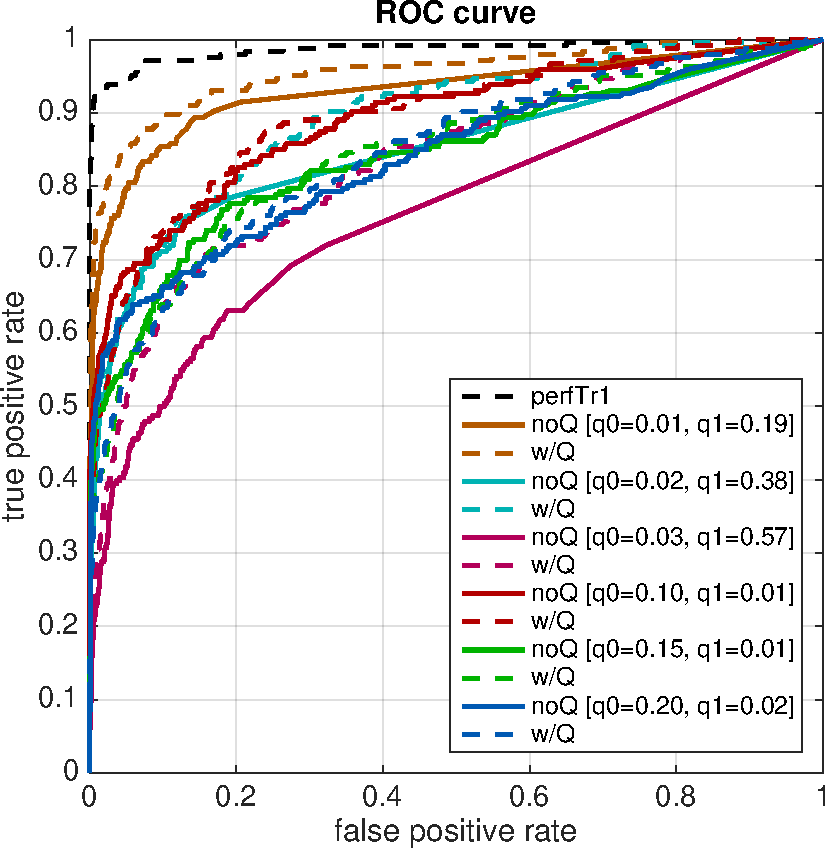
\includegraphics[width=10cm]{roc.pdf}
    \caption{Roc curves: variant noise levels - baseline vs. Q}
\end{figure}

\begin{figure}[H]
    \centering
    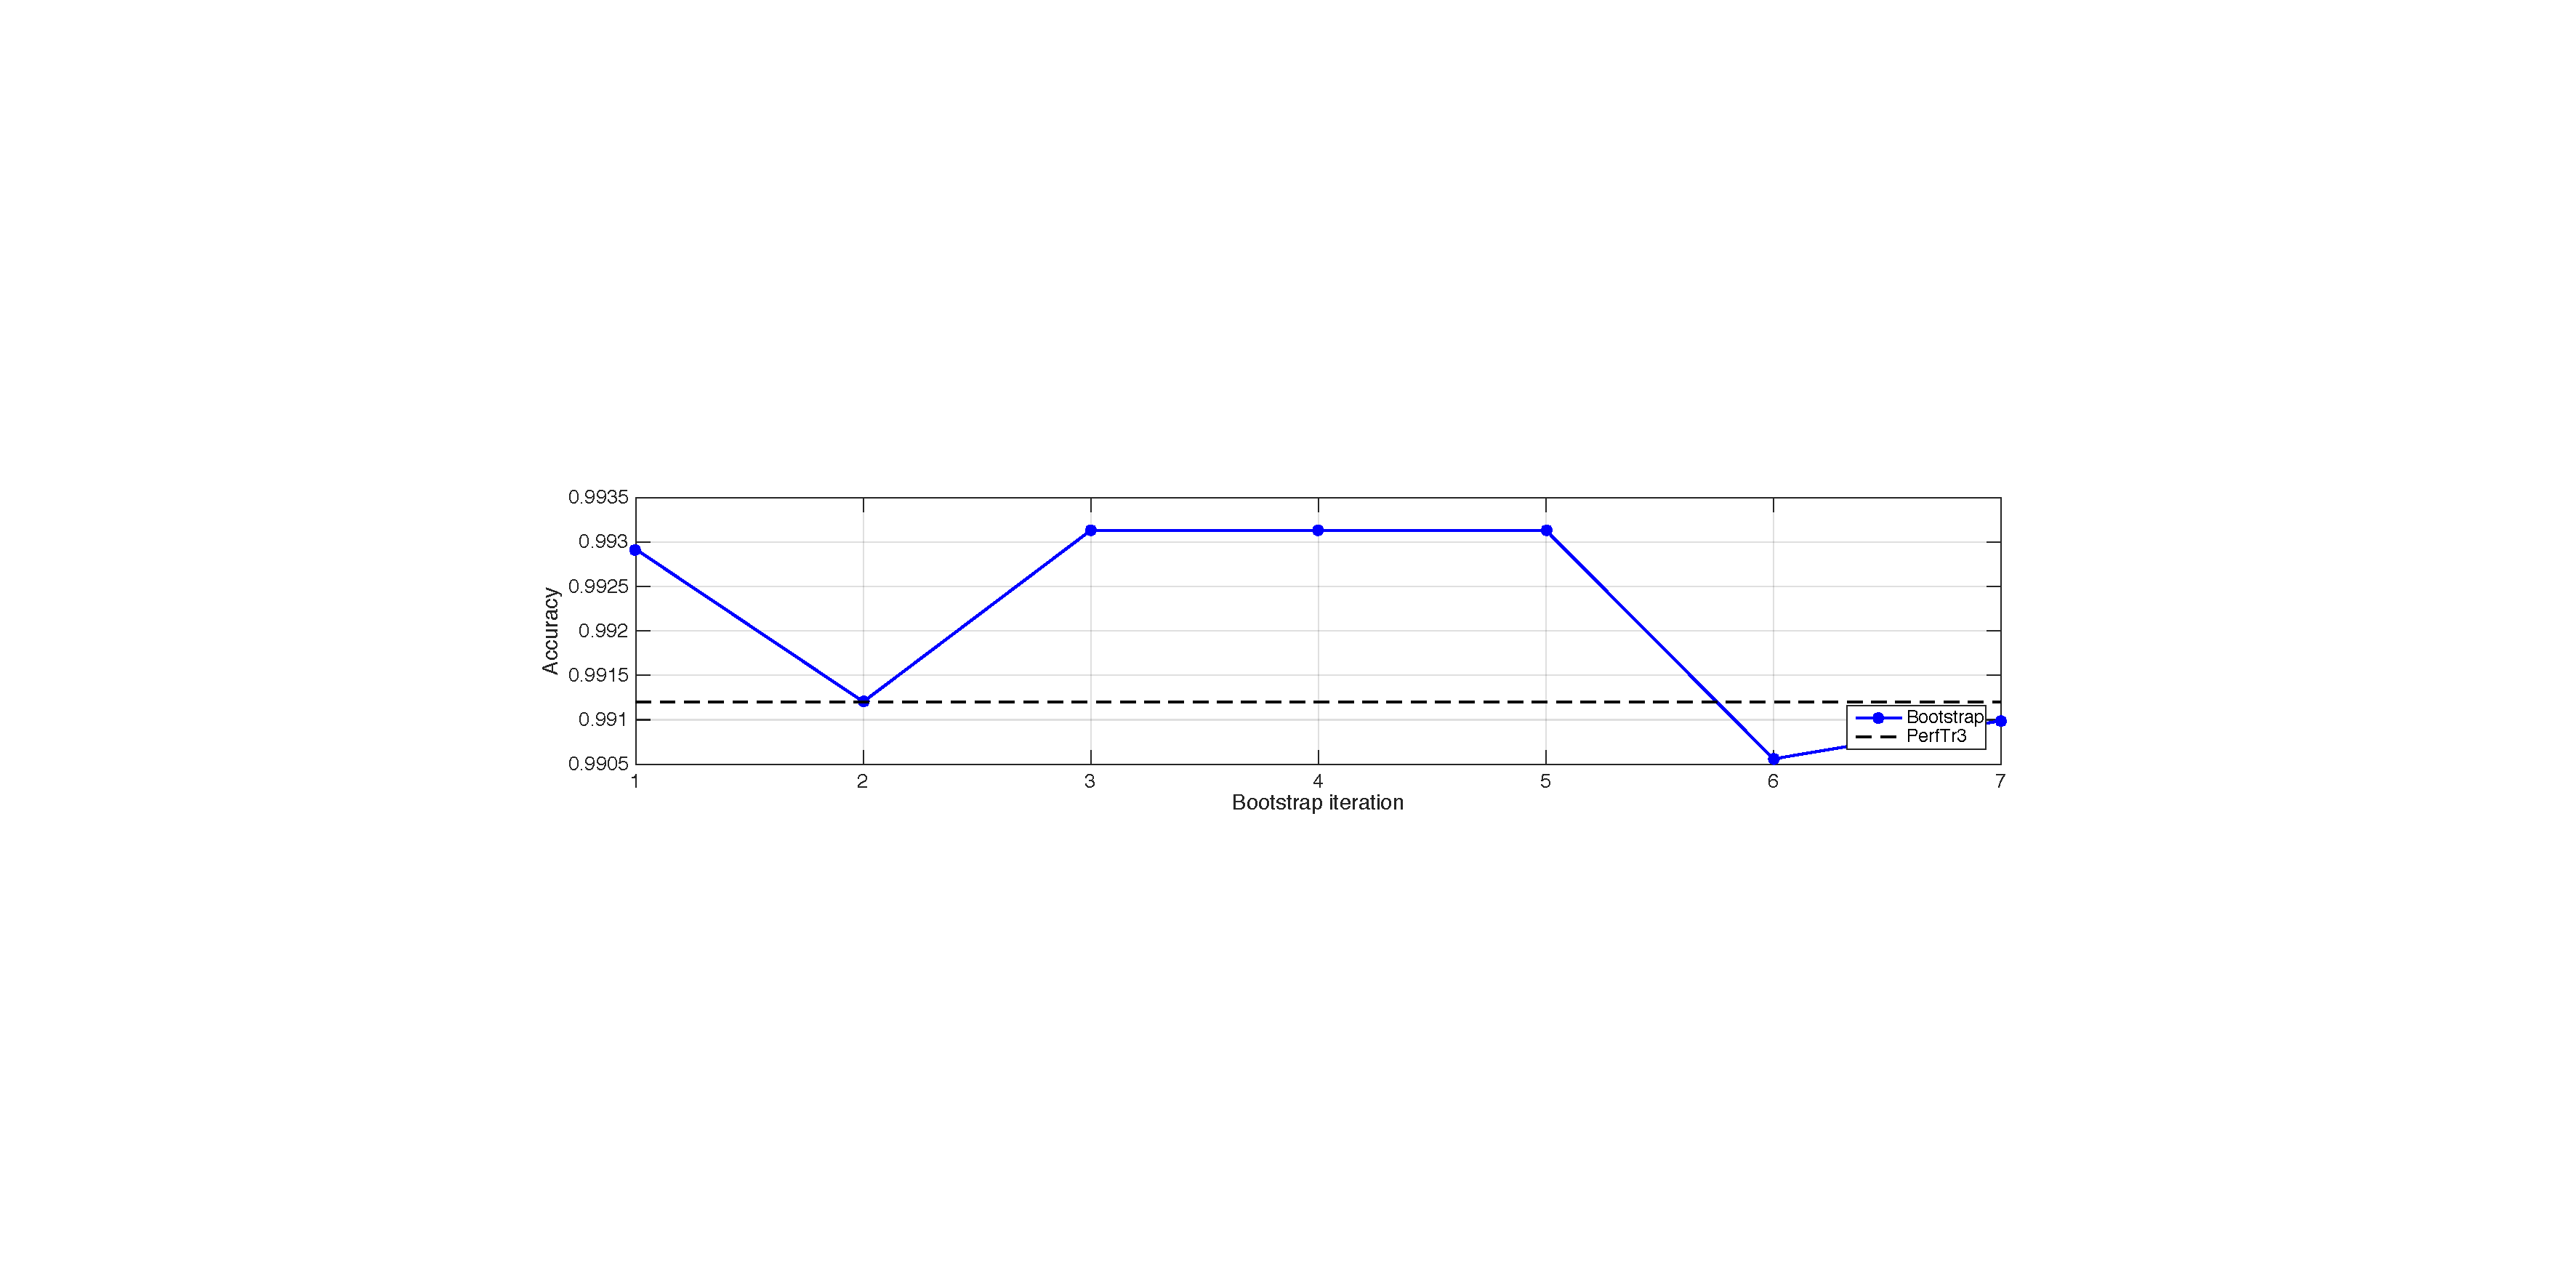
\includegraphics[width=16cm]{acc.pdf}
    \caption{Accuracies: variant noise levels - baseline vs. Q}
\end{figure}

\newpage
\section{Image dependent noise}
Thresholding the old classifier scores : 0 if score $<$ th1 , 1 if score $>$ th2\\
N1:  th1 = 10, th2 = 30\\
N2:  th1 = th2 = 20\\
N3:  th1 = th2 = 30\\
N3:  th1 = th2 = 40\\
\begin{table}[H]
\centering
\begin{tabular}{|c|c|c|c|c|c|c|c|}
\hline
              &$Test$ &$Train^{(s)}$ & $Train^{(f)}$ & N1        & N2       & N3      &  N4\\
\hline
     size     & 4661   &4152         & 381949          & 249683  & 381916   & 381942  &  381947\\
\textbf{1}    & 246    &214          & -               & 15862   & 32132    & 15827   &  10079\\
\textbf{0}    & 4415   &3938         & -               & 233821  & 349784   & 366115  &  371868\\
\textbf{(1)\%}& 5.3\%  & 5\%         & -               & 6.35\%  & 8.41\%   & 4.14\%  &  2.64\%\\

\hline
\end{tabular}
\end{table}
\begin{figure}[H]
    \centering
    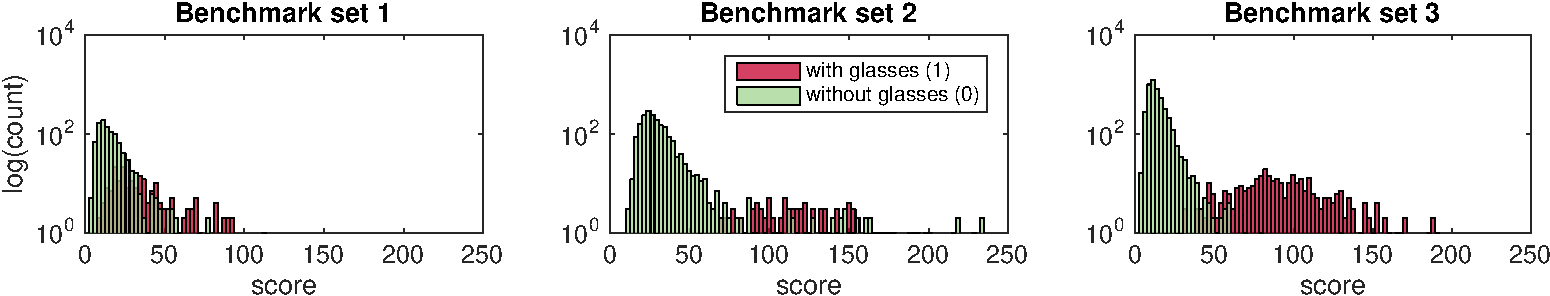
\includegraphics[width=12cm]{benchmark}
    \caption{Benchamrk dataset}
\end{figure}
\begin{figure}[H]
    \centering
    \includegraphics[width=12cm]{dataset}
    \caption{Training dataset}
\end{figure}
We estimate Q on a hand-labeled subset $Train^{(s)}\subset Train^{(f)}$
\begin{center}
$Q_1=\begin{pmatrix}.979&.021\\.08&.92\end{pmatrix}$
$Q_2=\begin{pmatrix}.9502&.0498\\.2103&.7897\end{pmatrix}$
$Q_3=\begin{pmatrix}.9963&.0037\\.3925&.6075\end{pmatrix}$
$Q_4=\begin{pmatrix}.9952&.0048\\.5447&.4553\end{pmatrix}$
\end{center}
Training for 10000 iters ($\approx$ 2 epochs):
\begin{figure}[H]
    \centering
    \includegraphics[width=16cm]{acc_im.pdf}
    \caption{Accuracies: baseline vs. Q}
\end{figure}
\begin{figure}[H]
    \centering
    \includegraphics[width=12cm]{roc_im2.pdf}
    \caption{Roc curves: baseline vs. Q}
\end{figure}
\begin{figure}[H]
    \centering
    \includegraphics[width=12cm]{roc_im_bis.pdf}
    \caption{Roc curves: baseline N1 -N2 -N3}
\end{figure}


\newpage
Training for 10000 iters ($\approx$ 2 epochs) - Then tuning w/Q for 10000 iters:

\begin{figure}[H]
    \centering
    \includegraphics[width=12cm]{roc_tuning2.pdf}
\end{figure}
\begin{figure}[H]
    \centering
    \includegraphics[width=12cm]{roc_tuning_bis.pdf}
    \caption{Roc curves: tuning N1 - N2 - N3}
\end{figure}

\begin{figure}[H]
    \centering
    \includegraphics[width=16cm]{acc_tuning.pdf}
    \caption{Accuracies - varying the thresholds + tuning w/Q}
\end{figure}

\section{Clean datasets}
C1: Multimedia Lab @Hong Kong\\
C2: $Train^{(s)}$
\begin{table}[H]
\centering
\begin{tabular}{|c|cc|}
\hline
           & C1   & C2: $Train^{(s)}$\\
\hline
Size       & 4151 &  4152  \\
\textbf{0} & 3362 &  3838   \\
\textbf{1} &  789 &   214   \\
\textbf{(1)\%}& 19\% & 5\%  \\
\hline
\end{tabular}
\end{table}
Test information loss with $Q_1=\begin{pmatrix}.99&.01\\.19&.81\end{pmatrix}$
\begin{figure}[H]
    \centering
    \includegraphics[width=12cm]{dclean}
    \caption{Roc curves - Clean training sets}
\end{figure}

\section{Balancing the datasets}
\textbf{For N1, N2 \& N3, we randomly choose 4$\times$ number of 1s from the 0' samples.}


\begin{figure}[H]
    \centering
    \includegraphics[width=16cm]{acc_balanced}
    \caption{Accuracies}
\end{figure}

\begin{figure}[H]
    \centering
    \includegraphics[width=12cm]{roc_baseline_balanced}
    \caption{Roc curves - baseline model 5\% vs 20\%}
\end{figure}

\begin{figure}[H]
    \centering
    \includegraphics[width=12cm]{roc_tuning_balanced}
    \caption{Roc curves - tuning w/ Q}
\end{figure}

\begin{figure}[H]
    \centering
    \includegraphics[width=12cm]{roc_infogain_balanced}
    \caption{Roc curves - Learning w/ Q}
\end{figure}

\begin{figure}[H]
    \centering
    \includegraphics[width=16cm]{roc_recap}
    \caption{Roc curves - comparison}
\end{figure}
\textbf{For N1, N2 \& N3, we randomly choose 1$\times$ number of 1s from the 0' samples.}\\
Baseline: batch loss $+\infty$
\begin{figure}[H]
    \centering
    \includegraphics[width=16cm]{acc_fifty}
    \caption{Accuracies}
\end{figure}

\begin{figure}[H]
    \centering
    \includegraphics[width=12cm]{roc_baseline_fifty}
    \caption{Roc curves - baseline model 5\% vs 50\% - baseline roc$\equiv 0$}
\end{figure}

\begin{figure}[H]
    \centering
    \includegraphics[width=12cm]{roc_infogain_fifty}
    \caption{Roc curves - 50\% Learning w/ Q}
\end{figure}
\end{document}


\newpage
\subsection{Fixing the baseline:}
(1) Larger batch $(64\rightarrow 120)$.\\
(2) Larger batch + batch normalization + w/o dropout.
\begin{figure}[H]
    \centering
    \includegraphics[width=12cm]{fix_baseline_acc}
    \caption{Accuracies}
\end{figure}
\begin{figure}[H]
    \centering
    \includegraphics[width=12cm]{fix_baseline_roc}
    \caption{Roc curves}
\end{figure}

